\section{Exposing and Mitigating Biases in Code Generation}

% Slide 10: Code Opener
\begin{frame}{In code, the shortcuts live in the prompt}
  \begin{itemize}
    \item Function names leak the solution
    \item Keywords act as hidden hints
    \item Examples do the reasoning for the model
    \item Question: Is the model solving, or pattern-matching?
  \end{itemize}
  \begin{center}
    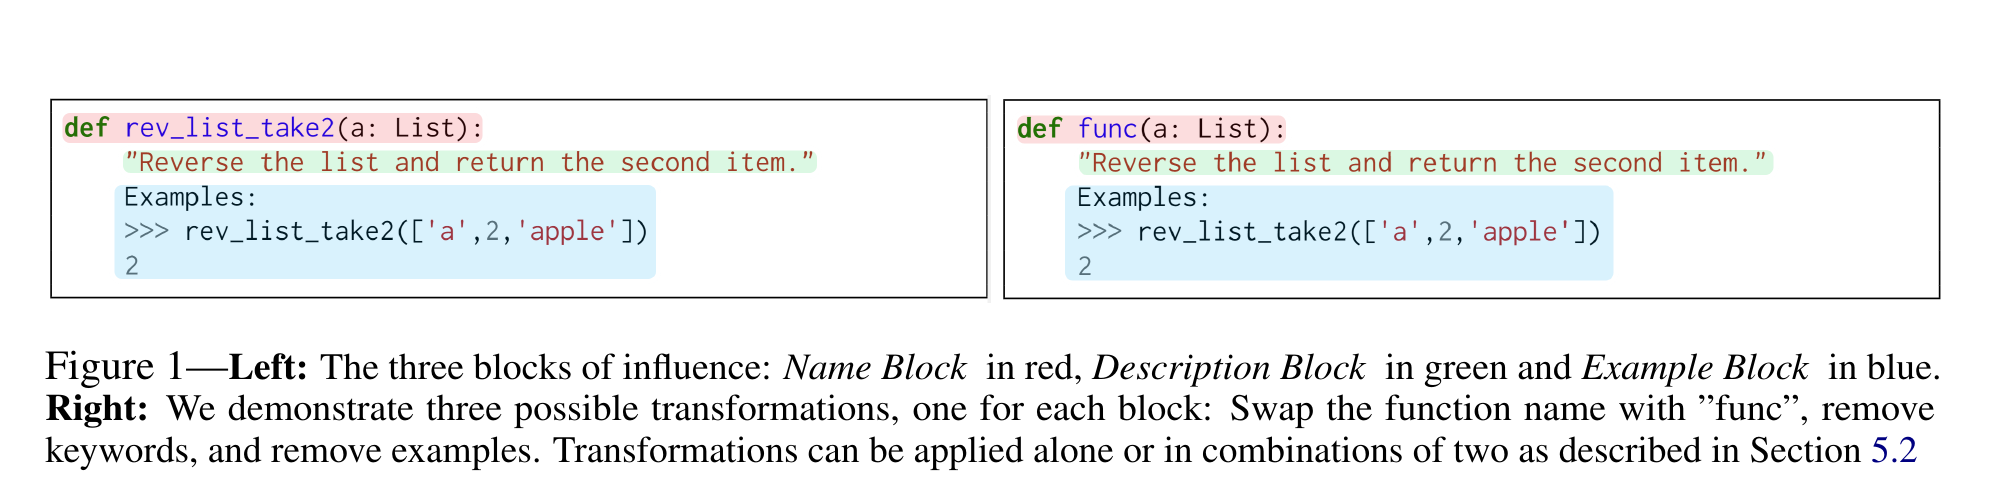
\includegraphics[width=0.8\textwidth,height=0.5\textheight,keepaspectratio]{assets/code-prompt-example}
    \vspace{-0.3em}
    {\tiny Source: Code prompt example (ACL 2023)}
  \end{center}
  \note{Chapter 3 is the language-domain continuation of the same idea. In vision, the shortcut can live in the scene. In code generation, the shortcut often lives in the prompt itself. Function names, task wording, and examples can all act as hidden hints. So I apply the same black-box semantic testing logic, but now to structured prompts instead of structured scenes.}
\end{frame}

% Slide 11: Blocks of Influence
\begin{frame}{Three blocks, three biases}
  \begin{columns}
    \column{0.48\textwidth}
    \begin{itemize}
      \item Name Block $\rightarrow$ memorization
      \item Description Block $\rightarrow$ lexical cue dependence
      \item Example Block $\rightarrow$ reasoning tie-breaker
      \item Perturb the blocks while preserving global task meaning
    \end{itemize}

    \column{0.52\textwidth}
    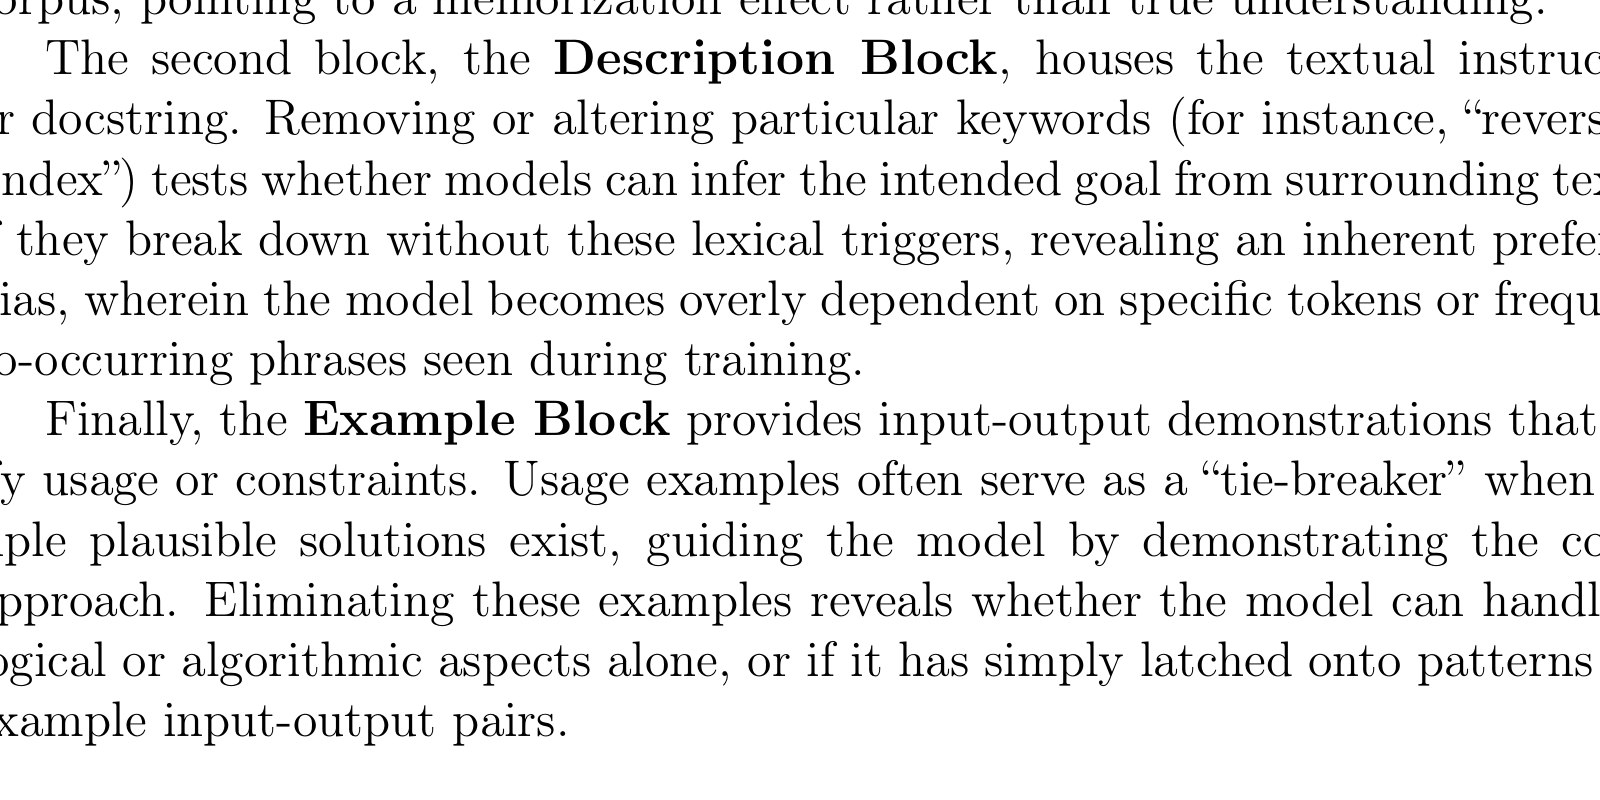
\includegraphics[width=\textwidth,height=0.6\textheight,keepaspectratio]{assets/thesis-fig-3-1-blocks-of-influence}
    \vspace{-0.3em}
    {\tiny Source: Thesis Fig. 3.1 / ACL 2023 Fig. 1}
  \end{columns}
  \note{This is the central abstraction of the code paper. I decompose the prompt into three Blocks of Influence. If renaming the function breaks performance, that suggests memorization. If removing a few keywords breaks it, that suggests lexical dependence. If removing examples breaks it, then the examples were doing reasoning work for the model. The important point is the task remains human-solvable after these transformations.}
\end{frame}

% Slide 12: Hero Slide — Remove the hints, lose the reasoning
\begin{frame}{Remove the hints, lose the reasoning}
  \begin{columns}[T]
    \column{0.31\textwidth}
    \begin{beamercolorbox}[wd=\linewidth,sep=1em,center]{block body}
      {\Large Anonymization}\\[1em]
      {\Huge \textbf{$\sim$19\%}}\\[0.5em]
      {\large drop}
    \end{beamercolorbox}

    \column{0.31\textwidth}
    \begin{beamercolorbox}[wd=\linewidth,sep=1em,center]{block body}
      {\Large Drop Keywords}\\[1em]
      {\Huge \textbf{$\sim$22\%}}\\[0.5em]
      {\large drop}
    \end{beamercolorbox}

    \column{0.31\textwidth}
    \begin{beamercolorbox}[wd=\linewidth,sep=1em,center]{block body}
      {\Large Combined}\\[1em]
      {\Huge \textbf{$\sim$40\%}}\\[0.5em]
      {\large drop}
    \end{beamercolorbox}
  \end{columns}

  \vspace{2em}
  \begin{center}
    {\Large The model was using the shortcuts, not solving the problem}
  \end{center}

  \note{This is the punch line of the code chapter. When I remove function-name hints via anonymization, performance drops by about 19 percent. When I remove selected keywords, it drops by about 22 percent. And when I combine those transformations, the drop reaches around 40 percent. The model was not reasoning from first principles. It was leaning on lexical and structural cues embedded in the prompt. Remove the scaffolding, and the reasoning collapses.}
\end{frame}

% Slide 13: Code Failures
\begin{frame}{Plausible code $\neq$ correct reasoning}
  \begin{itemize}
    \item Models often retain fragments of the right idea
    \item What fails is composition
    \item Still uses right operators, still looks intelligent, but logic is wrong
  \end{itemize}
  \begin{center}
    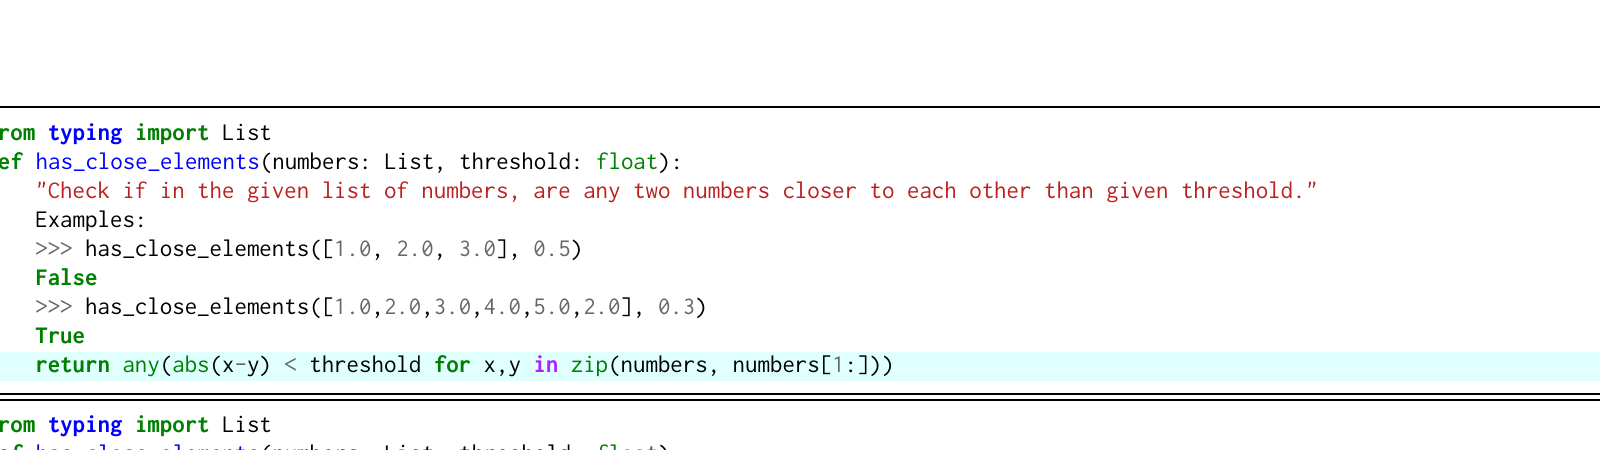
\includegraphics[width=0.85\textwidth,height=0.5\textheight,keepaspectratio]{assets/thesis-fig-3-2-code-single-example}
    \vspace{-0.3em}
    {\tiny Source: Thesis Fig. 3.2 (one before/after example)}
  \end{center}
  \note{These qualitative examples are very revealing. The model still produces code that looks intelligent and relevant. It may still compare numbers, iterate, or use the right operators. But it fails to compose those pieces into the correct algorithm. So the failure is not total ignorance. It is shallow reasoning hidden behind plausible code.}
\end{frame}

% Slide 14: Mitigation
\begin{frame}{Mitigation helps, but the bias remains}
  \begin{columns}
    \column{0.5\textwidth}
    \begin{itemize}
      \item Adversarial fine-tuning partially improves robustness
      \item Longer, richer descriptions help some models
      \item Larger models benefit more
      \item Bottom line: Partial improvement, not full solution
    \end{itemize}

    \column{0.5\textwidth}
    % Showing mitigation results (ACL Tables 4-5)
    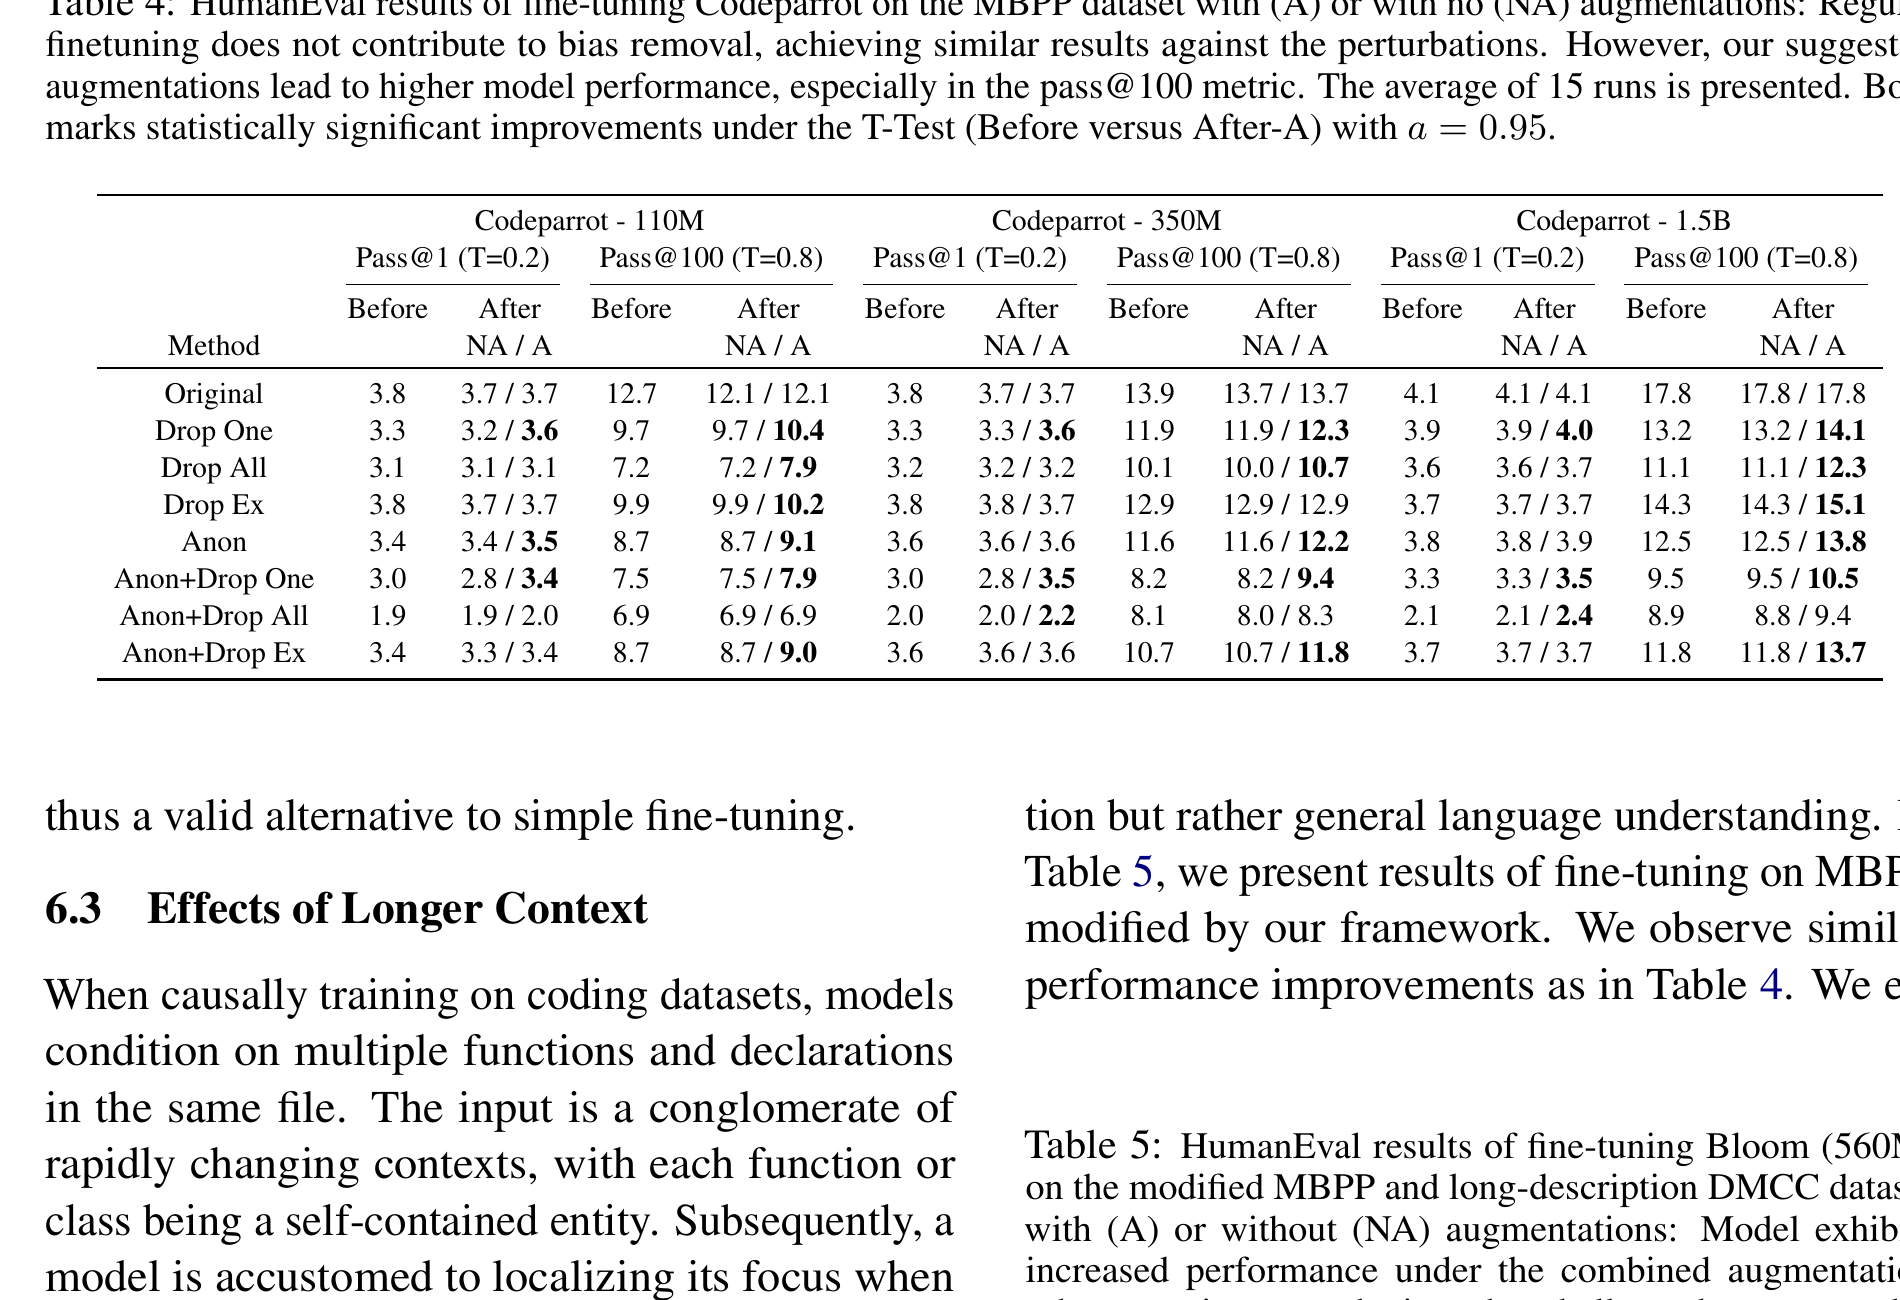
\includegraphics[width=\textwidth]{assets/acl-tables-4-5-cropped}
    \vspace{-0.3em}
    {\tiny Source: ACL 2023 Table 5 (fine-tuning results)}
  \end{columns}
  \note{I did not want this chapter to end only with diagnosis. So I used the perturbations as training augmentations. That helped, especially for larger models, and longer descriptions also improved resilience in some cases. But the gains were partial. The main conclusion stayed the same: data augmentation helps, but it does not fully remove the underlying shortcut dependence. This also serves as the cross-domain synthesis point. We now have the same pattern appearing in two completely different modalities. In vision, the shortcuts were spatial and configurational. In code, they are lexical and structural. But the underlying pathology is identical: models retreat to the easiest available signal when reasoning becomes hard.}
\end{frame}
